% Mars Survival Map -- presentation (Red Circle team). Build: pdflatex slides.tex (twice).
% Put real screenshots in figs/ with these names: map2d.png, map3d.png, safety.png, globe.png, overview.png
% A missing figure is replaced by a labelled box, so the deck always compiles.
\documentclass[aspectratio=169,11pt]{beamer}
\usepackage[utf8]{inputenc}
\usepackage[T1]{fontenc}
\usepackage{lmodern,amsmath,booktabs,tikz,graphicx}
\usetikzlibrary{arrows.meta,positioning}
\definecolor{leaf}{HTML}{4A9A2F}\definecolor{sky}{HTML}{2F9BE0}\definecolor{marsred}{HTML}{B8432A}
\definecolor{sun}{HTML}{F0BF2B}\definecolor{crimson}{HTML}{A1162F}\definecolor{ember}{HTML}{EC7A2C}\definecolor{violet}{HTML}{6A3FA8}
\definecolor{ink}{HTML}{1B2540}
\setbeamercolor{structure}{fg=violet}\setbeamercolor{title}{fg=ink}\setbeamercolor{frametitle}{fg=ink}
\setbeamercolor{normal text}{fg=ink}
\setbeamertemplate{navigation symbols}{}
\setbeamertemplate{footline}{\hfill\scriptsize\color{ink!60}Red Circle -- Mars Survival Map \quad \insertframenumber\hspace{4mm}\vspace{3mm}}
\setbeamertemplate{itemize item}{\color{marsred}$\bullet$}
\newcommand{\hyp}[1]{\textcolor{marsred}{\textbf{#1}}}
\newcommand{\fig}[2]{\IfFileExists{figs/#1.png}{\includegraphics[width=#2]{figs/#1.png}}{\fbox{\parbox[c][3.6cm][c]{#2}{\centering\small\color{ink!60}screenshot: figs/#1.png}}}}

\title{\textbf{Mars Survival Map}}
\subtitle{Where, and how, can a person on foot survive on Mars?}
\author{Red Circle team -- Douala}
\institute{NASA Space Apps 2026 -- Interplanetary Survival Guide: Martian Map}
\date{}

\begin{document}
\begin{frame}\titlepage\end{frame}

\begin{frame}{The question}
\begin{itemize}
\item A crew lands. \textbf{Where can they live, and which way can they walk and still get home?}
\item Existing Mars maps show terrain; none turns it into \textbf{survival decisions}: energy, time, cold, radio, shadow.
\item Our answer: one open web map, at three scales, with \textbf{every number traceable} to a source or declared a hypothesis.
\end{itemize}
\end{frame}

\begin{frame}{Three scales, one interface}
\begin{columns}[T]
\column{.32\textwidth}\textbf{Globe}\\ 0.5$^\circ$ grid ($\approx$30 km)\\ partial survival score + data coverage per cell\\[2mm]\fig{globe}{\textwidth}
\column{.32\textwidth}\textbf{Overview}\\ whole Jezero region, 20 m/px\\ detail windows you can open\\[2mm]\fig{overview}{\textwidth}
\column{.32\textwidth}\textbf{Site}\\ metre scale: hazards, routes, safety, 3D\\[2mm]\fig{map2d}{\textwidth}
\end{columns}
\end{frame}

\begin{frame}{Real, open data only}
\small
\begin{tabular}{@{}lll@{}}\toprule
\textbf{Scale} & \textbf{Source} & \textbf{Gives us}\\\midrule
Site & HiRISE DTM (UA), 1 m native, 4 m in the map & slope, roughness, routes, 3D\\
Overview & USGS CTX DEM mosaic, 20 m/px & whole-crater hillshade\\
Site & Mars 2020 MEDA (PDS) & temperature, pressure at Jezero\\
Globe & MOLA, Odyssey neutrons, TES, MCS, dust & elevation, water proxy, thermal, dust\\
Physics & Minetti 2002, Cavagna 2000, Apollo 16 & energy cost, suit power\\
Clock & Allison \& McEwen 2000 & Mars local solar time\\\bottomrule
\end{tabular}

\vspace{2mm}No login, no paywall. Registry with URL, what was taken and status: \texttt{sources.json}.
\end{frame}

\begin{frame}{Pipeline: heavy work offline, light work in the browser}
\centering
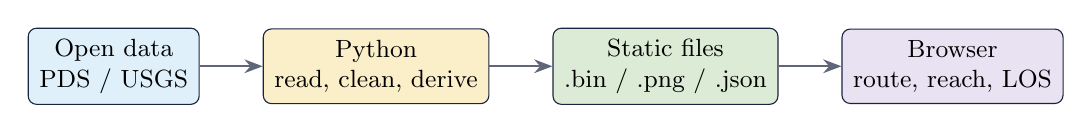
\begin{tikzpicture}[font=\small,node distance=8mm,box/.style={draw=ink,rounded corners=3pt,minimum height=9mm,align=center,inner sep=4pt},arr/.style={-{Stealth},thick,ink!70}]
\node[box,fill=sky!15] (a) {Open data\\PDS / USGS};
\node[box,fill=sun!25,right=of a] (b) {Python\\read, clean, derive};
\node[box,fill=leaf!20,right=of b] (c) {Static files\\.bin / .png / .json};
\node[box,fill=violet!15,right=of c] (d) {Browser\\route, reach, LOS};
\draw[arr](a)--(b);\draw[arr](b)--(c);\draw[arr](c)--(d);
\end{tikzpicture}
\begin{itemize}\small
\item A 700 MB DTM is read as a \textbf{6 km window with HTTP Range requests}, resumable when the server cuts the transfer.
\item Hosting is a plain static folder: no server, works offline after the first visit.
\end{itemize}
\end{frame}

\begin{frame}{What the terrain becomes}
\begin{itemize}
\item \textbf{Slope} and \textbf{roughness} from the DTM (roughness = local standard deviation after removing the slope plane, 60 m window).
\item \textbf{Four hazard classes}: safe, caution, hazardous, forbidden (slope 10/20/25$^\circ$, roughness 0.25/0.6/1.5 m) \hyp{team assumptions}.
\item \textbf{Flat sites}: discs 120 m across with at most 5\% of pixels outside the limits.
\end{itemize}
\vspace{2mm}\centering\fig{map3d}{.55\textwidth}
\end{frame}

\begin{frame}{Least-energy routes}
Minetti (2002): cost of walking vs.\ grade $i$,
\[C_w(i)=280.5i^5-58.7i^4-76.8i^3+51.9i^2+19.6i+2.5\ \ [\mathrm{J\,kg^{-1}m^{-1}}]\]
Mars gravity: $C_\text{Mars}(i)=0.75\,C_w(0)+\big(C_w(i)-C_w(0)\big)\,g_M/g_E$ \hyp{(hypothesis)}
\begin{itemize}
\item 8-connected graph, directed step cost $E=m\,C\,\ell\,\bar\mu$, Dijkstra with a binary heap, $O(N\log N)$.
\item Same algorithm in Python and JavaScript, \textbf{parity tested}.
\item Walking speed is a slider (1--40 km/h); slopes still slow the walker.
\end{itemize}
\end{frame}

\begin{frame}{Safety tools}
\begin{columns}[T]
\column{.5\textwidth}
\begin{itemize}
\item \textbf{Return to shelter}: out-and-back reach from forward and reverse cost fields; limits $T_\text{max}=8\,\text{h}\times(1-25\%)$, $E_\text{max}=272.6\,\text{W}\times T_\text{max}$.
\item \textbf{Radio line of sight} with Mars curvature.
\item \textbf{Shadows} by ray march along the sun azimuth.
\item \textbf{Time budget}: sunset, cold, safe start windows.
\end{itemize}
\column{.48\textwidth}\fig{safety}{\textwidth}
\end{columns}
\end{frame}

\begin{frame}{Walking it}
\begin{itemize}
\item \textbf{Simulated walker}: heading arrow, path wipes as you advance, turn-by-turn guidance, \emph{Correct my position}.
\item \textbf{Walker's view} (first person), \textbf{printable route card}, \textbf{saved places} (searchable), \textbf{offline mode}.
\item There is no GPS on Mars, so we say plainly that this is a simulation of the plan.
\end{itemize}
\end{frame}

\begin{frame}{Honesty is a feature}
\begin{columns}[T]
\column{.5\textwidth}\textbf{What is measured}
\begin{itemize}\small\item HiRISE elevation\item MEDA weather\item Neutron flux, thermal inertia\item Apollo suit power (on the Moon)\end{itemize}
\column{.5\textwidth}\textbf{What is a hypothesis} \hyp{(tagged in the UI)}
\begin{itemize}\small\item Gravity scaling of walking cost\item Hazard and roughness thresholds\item 25\% reserve, antenna heights\item Temperature as a sinusoid\end{itemize}
\end{columns}
\vspace{2mm}Each cell of the globe shows its \textbf{data coverage}; missing layers are never filled with invented values.
\end{frame}

\begin{frame}{Verification}
\begin{itemize}
\item \textbf{80 pytest} tests and Node tests (Mars clock; reach, line of sight, shadows, time budget).
\item Python/JavaScript \textbf{routing parity}; PDS3 reader tested against a server that cuts transfers.
\item Scripted browser runs: load, route, walk, no page errors.
\item Languages: English, French; Ewondo is wired in and waits for native speakers.
\end{itemize}
\end{frame}

\begin{frame}{Limits and next steps}
\begin{columns}[T]
\column{.5\textwidth}\textbf{Limits}
\begin{itemize}\small\item DTM too coarse for boulders\item One detail window so far\item Globe score is partial\item Walking model is an Earth measurement\end{itemize}
\column{.5\textwidth}\textbf{Next}
\begin{itemize}\small\item More detail windows (Gale, others)\item USGS TRN DTM with a confidence layer\item Rock and wind layers\item Published MEDA temperature fits\end{itemize}
\end{columns}
\end{frame}

\begin{frame}[plain]
\centering\vspace{1.2cm}{\Huge\textbf{Thank you}}\\[6mm]
{\large Red Circle -- Douala}\\[4mm]
\small Source code, data registry and technical report included.
\end{frame}
\end{document}
